\documentclass{standalone}
\usepackage{tikz}
\usetikzlibrary{patterns, positioning}
\usepackage[sfdefault]{ClearSans} %% option 'sfdefault' activates Clear Sans as the default text font
\usepackage[T1]{fontenc}

\begin{document}
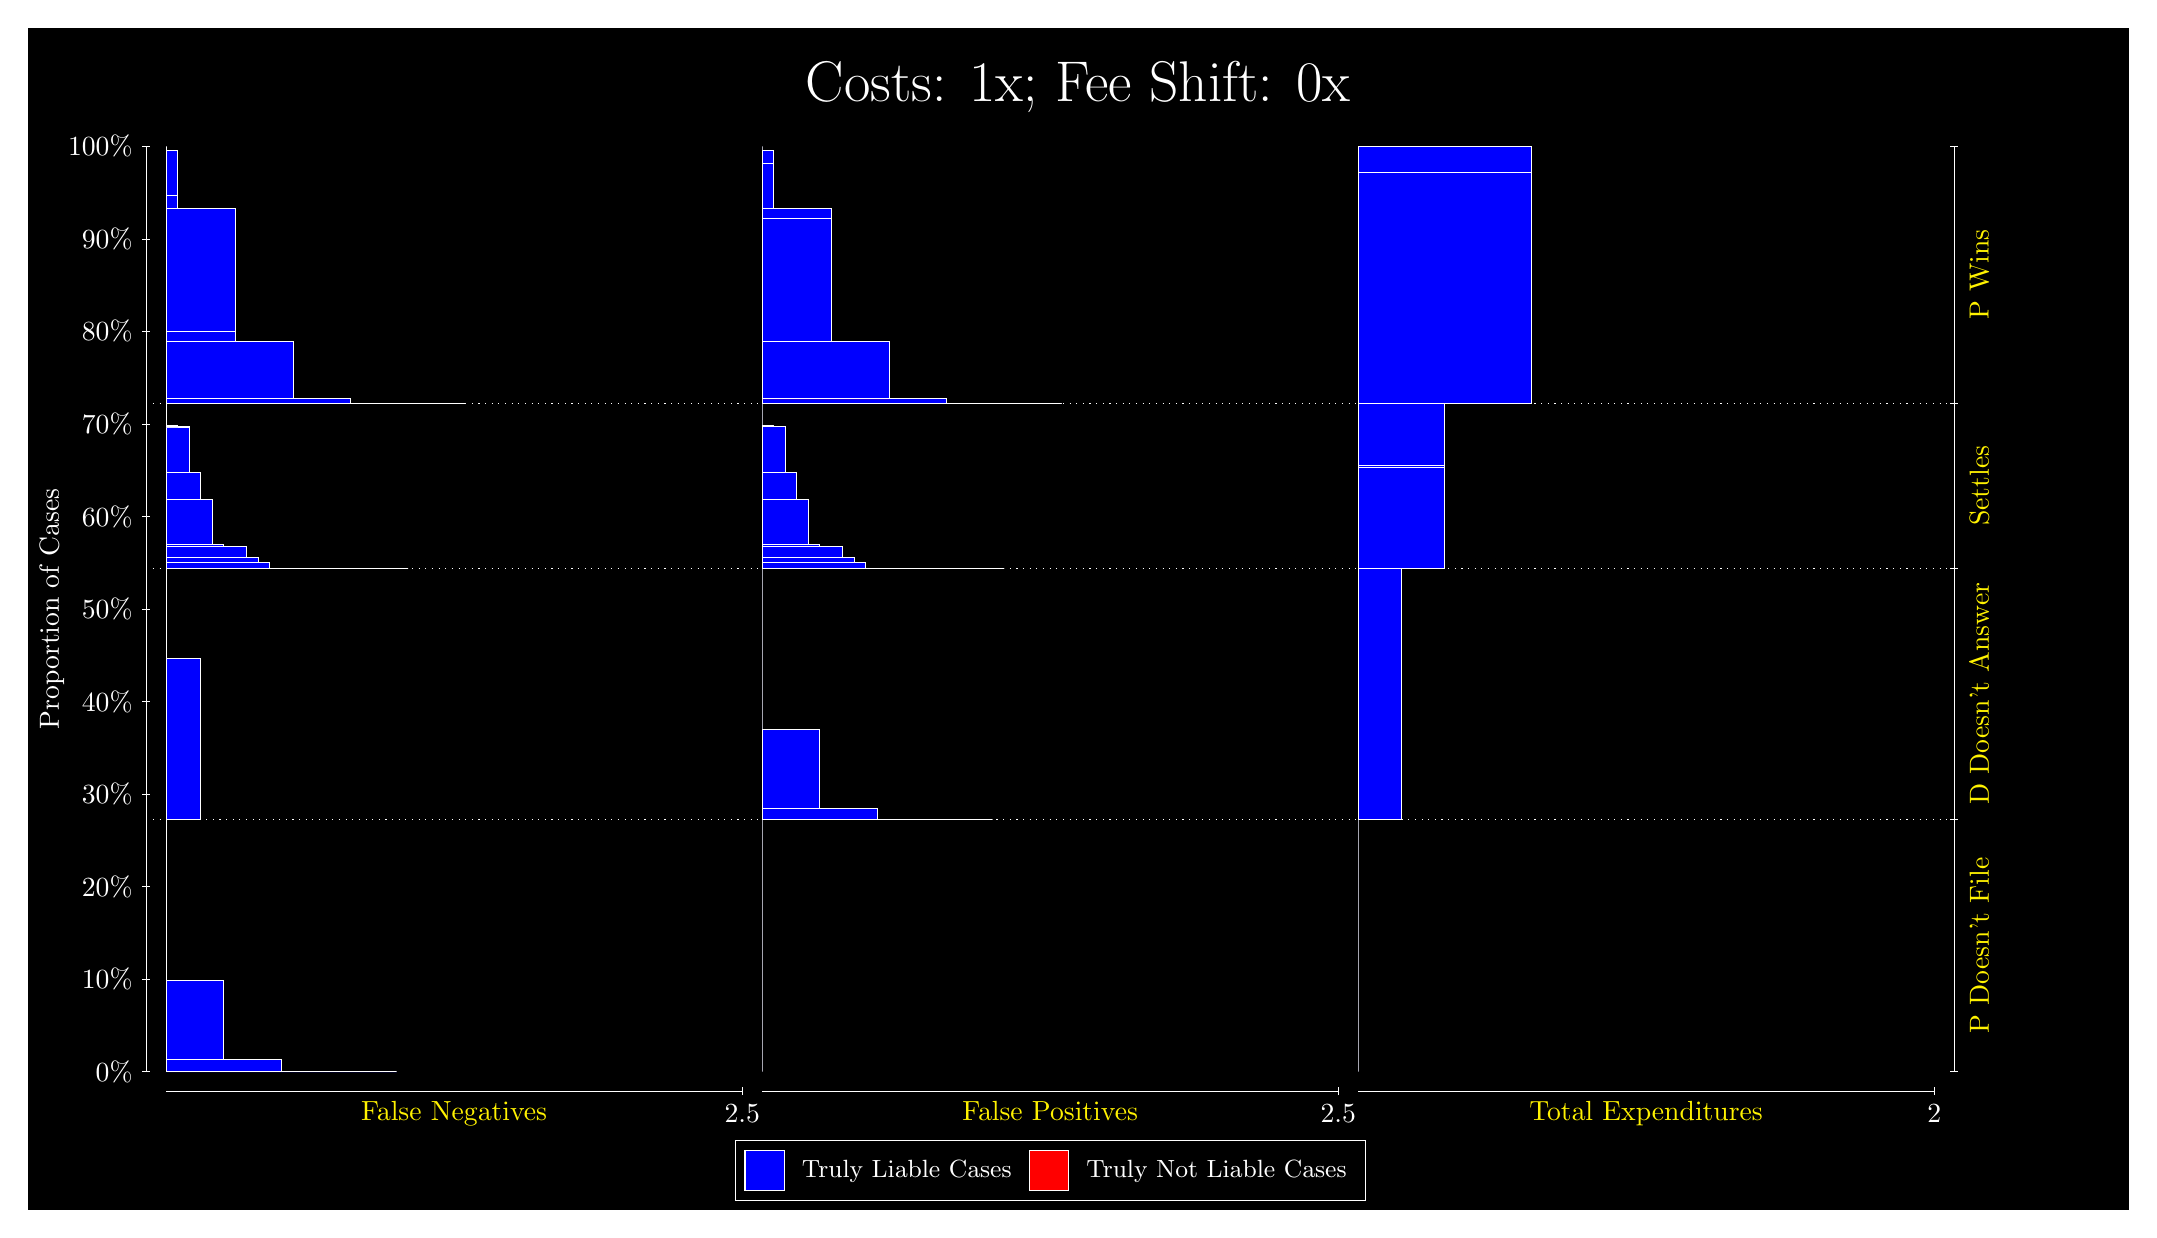
\begin{tikzpicture}
\draw[fill=black] (0,0) rectangle (26.667,15);
\draw[text=white] (0,13.5) rectangle (26.667,15) node[midway] {\huge Costs: 1x; Fee Shift: 0x};
\draw[white, very thin] (1.5,1.75) -- (1.5,13.5);
\node[rotate=90, text=white, anchor=center] at (0.3, 7.625) {Proportion of Cases};
\draw[white, very thin] (1.45,1.75) -- (1.55,1.75);
\node[text=white, anchor=east] at (1.45, 1.75) {0\%};
\draw[white, very thin] (1.45,2.925) -- (1.55,2.925);
\node[text=white, anchor=east] at (1.45, 2.925) {10\%};
\draw[white, very thin] (1.45,4.1) -- (1.55,4.1);
\node[text=white, anchor=east] at (1.45, 4.1) {20\%};
\draw[white, very thin] (1.45,5.275) -- (1.55,5.275);
\node[text=white, anchor=east] at (1.45, 5.275) {30\%};
\draw[white, very thin] (1.45,6.45) -- (1.55,6.45);
\node[text=white, anchor=east] at (1.45, 6.45) {40\%};
\draw[white, very thin] (1.45,7.625) -- (1.55,7.625);
\node[text=white, anchor=east] at (1.45, 7.625) {50\%};
\draw[white, very thin] (1.45,8.8) -- (1.55,8.8);
\node[text=white, anchor=east] at (1.45, 8.8) {60\%};
\draw[white, very thin] (1.45,9.975) -- (1.55,9.975);
\node[text=white, anchor=east] at (1.45, 9.975) {70\%};
\draw[white, very thin] (1.45,11.15) -- (1.55,11.15);
\node[text=white, anchor=east] at (1.45, 11.15) {80\%};
\draw[white, very thin] (1.45,12.325) -- (1.55,12.325);
\node[text=white, anchor=east] at (1.45, 12.325) {90\%};
\draw[white, very thin] (1.45,13.5) -- (1.55,13.5);
\node[text=white, anchor=east] at (1.45, 13.5) {100\%};

\draw[white, very thin] (24.457,1.75) -- (24.457,13.5);
\draw[white, very thin] (24.407,1.75) -- (24.507,1.75);
\node[anchor=west] at (24.407, 1.75) {};
\draw[white, very thin] (24.407,4.9531) -- (24.507,4.9531);
\node[anchor=west] at (24.407, 4.9531) {};
\draw[white, very thin] (24.407,8.143) -- (24.507,8.143);
\node[anchor=west] at (24.407, 8.143) {};
\draw[white, very thin] (24.407,10.239) -- (24.507,10.239);
\node[anchor=west] at (24.407, 10.239) {};
\draw[white, very thin] (24.407,13.5) -- (24.507,13.5);
\node[anchor=west] at (24.407, 13.5) {};

\draw[white, very thin, fill=blue] (1.75,1.75) rectangle (4.6775,1.75);
\draw[white, very thin, fill=blue] (1.75,1.75) rectangle (3.9457,1.7513);
\draw[white, very thin, fill=blue] (1.75,1.7513) rectangle (3.2138,1.9023);
\draw[white, very thin, fill=blue] (1.75,1.9023) rectangle (2.4819,2.9078);
\draw[white, very thin, fill=red] (1.75,2.9078) rectangle (1.75,2.9078);
\draw[white, very thin, fill=blue] (1.75,2.9078) rectangle (1.75,4.9531);
\draw[white, very thin, fill=blue] (1.75,4.9531) rectangle (2.1891,6.9984);
\draw[white, very thin, fill=red] (1.75,6.9984) rectangle (1.75,6.9984);
\draw[white, very thin, fill=blue] (1.75,6.9984) rectangle (1.75,8.143);
\draw[white, very thin, fill=blue] (1.75,8.143) rectangle (4.8239,8.143);
\draw[white, very thin, fill=blue] (1.75,8.143) rectangle (4.5312,8.143);
\draw[white, very thin, fill=blue] (1.75,8.143) rectangle (4.2384,8.143);
\draw[white, very thin, fill=blue] (1.75,8.143) rectangle (4.092,8.143);
\draw[white, very thin, fill=blue] (1.75,8.143) rectangle (3.9457,8.143);
\draw[white, very thin, fill=blue] (1.75,8.143) rectangle (3.7993,8.143);
\draw[white, very thin, fill=blue] (1.75,8.143) rectangle (3.6529,8.1431);
\draw[white, very thin, fill=blue] (1.75,8.1431) rectangle (3.5065,8.1433);
\draw[white, very thin, fill=blue] (1.75,8.1433) rectangle (3.3602,8.1433);
\draw[white, very thin, fill=blue] (1.75,8.1433) rectangle (3.2138,8.1433);
\draw[white, very thin, fill=blue] (1.75,8.1433) rectangle (3.0674,8.2177);
\draw[white, very thin, fill=blue] (1.75,8.2177) rectangle (3.0674,8.2178);
\draw[white, very thin, fill=blue] (1.75,8.2178) rectangle (2.921,8.281);
\draw[white, very thin, fill=blue] (1.75,8.281) rectangle (2.7746,8.421);
\draw[white, very thin, fill=blue] (1.75,8.421) rectangle (2.6283,8.4211);
\draw[white, very thin, fill=blue] (1.75,8.4211) rectangle (2.6283,8.4219);
\draw[white, very thin, fill=blue] (1.75,8.4219) rectangle (2.4819,8.4433);
\draw[white, very thin, fill=blue] (1.75,8.4433) rectangle (2.3355,9.0132);
\draw[white, very thin, fill=blue] (1.75,9.0132) rectangle (2.3355,9.0196);
\draw[white, very thin, fill=blue] (1.75,9.0196) rectangle (2.1891,9.3628);
\draw[white, very thin, fill=blue] (1.75,9.3628) rectangle (2.0428,9.9324);
\draw[white, very thin, fill=blue] (1.75,9.9324) rectangle (2.0428,9.9388);
\draw[white, very thin, fill=blue] (1.75,9.9388) rectangle (1.8964,9.9388);
\draw[white, very thin, fill=blue] (1.75,9.9388) rectangle (1.8964,9.9603);
\draw[white, very thin, fill=blue] (1.75,9.9603) rectangle (1.75,9.9603);
\draw[white, very thin, fill=red] (1.75,9.9603) rectangle (1.75,9.9603);
\draw[white, very thin, fill=blue] (1.75,9.9603) rectangle (1.75,10.239);
\draw[white, very thin, fill=blue] (1.75,10.239) rectangle (5.5558,10.239);
\draw[white, very thin, fill=blue] (1.75,10.239) rectangle (4.8239,10.239);
\draw[white, very thin, fill=blue] (1.75,10.239) rectangle (4.092,10.294);
\draw[white, very thin, fill=blue] (1.75,10.294) rectangle (3.3602,11.021);
\draw[white, very thin, fill=blue] (1.75,11.021) rectangle (2.6283,11.149);
\draw[white, very thin, fill=blue] (1.75,11.149) rectangle (2.6283,12.717);
\draw[white, very thin, fill=blue] (1.75,12.717) rectangle (1.8964,12.883);
\draw[white, very thin, fill=blue] (1.75,12.883) rectangle (1.8964,13.445);
\draw[white, very thin, fill=red] (1.75,13.445) rectangle (1.75,13.445);
\draw[white, very thin, fill=blue] (1.75,13.445) rectangle (1.75,13.5);
\draw[white, very thin, fill=red] (9.3189,1.75) rectangle (9.3189,1.75);
\draw[white, very thin, fill=blue] (9.3189,1.75) rectangle (9.3189,4.9531);
\draw[white, very thin, fill=red] (9.3189,4.9531) rectangle (12.246,4.9531);
\draw[white, very thin, fill=blue] (9.3189,4.9531) rectangle (12.246,4.9531);
\draw[white, very thin, fill=blue] (9.3189,4.9531) rectangle (11.515,4.9538);
\draw[white, very thin, fill=blue] (9.3189,4.9538) rectangle (10.783,5.0927);
\draw[white, very thin, fill=blue] (9.3189,5.0927) rectangle (10.051,6.0977);
\draw[white, very thin, fill=blue] (9.3189,6.0977) rectangle (9.3189,8.143);
\draw[white, very thin, fill=red] (9.3189,8.143) rectangle (12.393,8.143);
\draw[white, very thin, fill=blue] (9.3189,8.143) rectangle (12.393,8.143);
\draw[white, very thin, fill=red] (9.3189,8.143) rectangle (12.1,8.143);
\draw[white, very thin, fill=blue] (9.3189,8.143) rectangle (12.1,8.143);
\draw[white, very thin, fill=red] (9.3189,8.143) rectangle (11.807,8.143);
\draw[white, very thin, fill=blue] (9.3189,8.143) rectangle (11.807,8.143);
\draw[white, very thin, fill=blue] (9.3189,8.143) rectangle (11.661,8.143);
\draw[white, very thin, fill=red] (9.3189,8.143) rectangle (11.515,8.143);
\draw[white, very thin, fill=blue] (9.3189,8.143) rectangle (11.515,8.143);
\draw[white, very thin, fill=blue] (9.3189,8.143) rectangle (11.368,8.143);
\draw[white, very thin, fill=red] (9.3189,8.143) rectangle (11.222,8.143);
\draw[white, very thin, fill=blue] (9.3189,8.143) rectangle (11.222,8.1431);
\draw[white, very thin, fill=blue] (9.3189,8.1431) rectangle (11.075,8.1433);
\draw[white, very thin, fill=blue] (9.3189,8.1433) rectangle (10.929,8.1433);
\draw[white, very thin, fill=red] (9.3189,8.1433) rectangle (10.929,8.1433);
\draw[white, very thin, fill=blue] (9.3189,8.1433) rectangle (10.929,8.1433);
\draw[white, very thin, fill=blue] (9.3189,8.1433) rectangle (10.783,8.1433);
\draw[white, very thin, fill=blue] (9.3189,8.1433) rectangle (10.636,8.1434);
\draw[white, very thin, fill=red] (9.3189,8.1434) rectangle (10.636,8.1434);
\draw[white, very thin, fill=blue] (9.3189,8.1434) rectangle (10.636,8.2174);
\draw[white, very thin, fill=blue] (9.3189,8.2174) rectangle (10.49,8.2806);
\draw[white, very thin, fill=red] (9.3189,8.2806) rectangle (10.344,8.2806);
\draw[white, very thin, fill=blue] (9.3189,8.2806) rectangle (10.344,8.4206);
\draw[white, very thin, fill=blue] (9.3189,8.4206) rectangle (10.197,8.4214);
\draw[white, very thin, fill=blue] (9.3189,8.4214) rectangle (10.197,8.4214);
\draw[white, very thin, fill=red] (9.3189,8.4214) rectangle (10.051,8.4214);
\draw[white, very thin, fill=blue] (9.3189,8.4214) rectangle (10.051,8.443);
\draw[white, very thin, fill=blue] (9.3189,8.443) rectangle (9.9044,8.4494);
\draw[white, very thin, fill=blue] (9.3189,8.4494) rectangle (9.9044,9.0189);
\draw[white, very thin, fill=blue] (9.3189,9.0189) rectangle (9.758,9.3622);
\draw[white, very thin, fill=blue] (9.3189,9.3622) rectangle (9.6116,9.9384);
\draw[white, very thin, fill=blue] (9.3189,9.9384) rectangle (9.4652,9.9599);
\draw[white, very thin, fill=blue] (9.3189,9.9599) rectangle (9.4652,9.9599);
\draw[white, very thin, fill=blue] (9.3189,9.9599) rectangle (9.3189,10.239);
\draw[white, very thin, fill=red] (9.3189,10.239) rectangle (13.125,10.239);
\draw[white, very thin, fill=blue] (9.3189,10.239) rectangle (13.125,10.239);
\draw[white, very thin, fill=red] (9.3189,10.239) rectangle (12.393,10.239);
\draw[white, very thin, fill=blue] (9.3189,10.239) rectangle (12.393,10.239);
\draw[white, very thin, fill=red] (9.3189,10.239) rectangle (11.661,10.239);
\draw[white, very thin, fill=blue] (9.3189,10.239) rectangle (11.661,10.294);
\draw[white, very thin, fill=red] (9.3189,10.294) rectangle (10.929,10.294);
\draw[white, very thin, fill=blue] (9.3189,10.294) rectangle (10.929,11.022);
\draw[white, very thin, fill=blue] (9.3189,11.022) rectangle (10.197,12.589);
\draw[white, very thin, fill=red] (9.3189,12.589) rectangle (10.197,12.589);
\draw[white, very thin, fill=blue] (9.3189,12.589) rectangle (10.197,12.717);
\draw[white, very thin, fill=blue] (9.3189,12.717) rectangle (9.4652,13.28);
\draw[white, very thin, fill=blue] (9.3189,13.28) rectangle (9.4652,13.445);
\draw[white, very thin, fill=blue] (9.3189,13.445) rectangle (9.3189,13.5);
\draw[white, very thin, fill=red] (16.888,1.75) rectangle (16.888,1.75);
\draw[white, very thin, fill=blue] (16.888,1.75) rectangle (16.888,4.9531);
\draw[white, very thin, fill=red] (16.888,4.9531) rectangle (17.437,4.9531);
\draw[white, very thin, fill=blue] (16.888,4.9531) rectangle (17.437,8.143);
\draw[white, very thin, fill=red] (16.888,8.143) rectangle (17.986,8.143);
\draw[white, very thin, fill=blue] (16.888,8.143) rectangle (17.986,9.4262);
\draw[white, very thin, fill=red] (16.888,9.4262) rectangle (17.986,9.4262);
\draw[white, very thin, fill=blue] (16.888,9.4262) rectangle (17.986,9.4486);
\draw[white, very thin, fill=red] (16.888,9.4486) rectangle (17.986,9.4486);
\draw[white, very thin, fill=blue] (16.888,9.4486) rectangle (17.986,10.239);
\draw[white, very thin, fill=red] (16.888,10.239) rectangle (19.083,10.239);
\draw[white, very thin, fill=blue] (16.888,10.239) rectangle (19.083,13.174);
\draw[white, very thin, fill=red] (16.888,13.174) rectangle (19.083,13.174);
\draw[white, very thin, fill=blue] (16.888,13.174) rectangle (19.083,13.5);
\draw[white, dotted] (1.5,4.9531) -- (24.457,4.9531);
\draw[white, dotted] (1.5,8.143) -- (24.457,8.143);
\draw[white, dotted] (1.5,10.239) -- (24.457,10.239);
\draw[white, very thin] (1.75,1.5) -- (9.0689,1.5);
\node[text=yellow, anchor=north] at (5.4094, 1.5) {False Negatives};
\draw[white, very thin] (9.0689,1.45) -- (9.0689,1.55);
\node[text=white, anchor=north] at (9.0689, 1.45) {2.5};

\draw[white, very thin] (9.3189,1.5) -- (16.638,1.5);
\node[text=yellow, anchor=north] at (12.978, 1.5) {False Positives};
\draw[white, very thin] (16.638,1.45) -- (16.638,1.55);
\node[text=white, anchor=north] at (16.638, 1.45) {2.5};

\draw[white, very thin] (16.888,1.5) -- (24.207,1.5);
\node[text=yellow, anchor=north] at (20.547, 1.5) {Total Expenditures};
\draw[white, very thin] (24.207,1.45) -- (24.207,1.55);
\node[text=white, anchor=north] at (24.207, 1.45) {2};

\node[text=yellow, centered, rotate=90] at (24.777, 3.3516) {P Doesn't File};
\node[text=yellow, centered, rotate=90] at (24.777, 6.548) {D Doesn't Answer};
\node[text=yellow, centered, rotate=90] at (24.777, 9.1909) {Settles};
\node[text=yellow, centered, rotate=90] at (24.777, 11.869) {P Wins};

\draw (12.978300999999998,1.5) node[draw=none] (baseCoordinate) {};
\begin{scope}[align=center]
        \matrix[scale=0.5, draw=white, below=0.5cm of baseCoordinate, nodes={draw}, column sep=0.1cm]{
            \node[rectangle, draw, minimum width=0.5cm, minimum height=0.5cm, fill=blue] {}; &
            \node[draw=none, font=\small, text=white] (B) {Truly Liable Cases}; &
            \node[rectangle, draw, minimum width=0.5cm, minimum height=0.5cm, fill=red] {}; &
            \node[draw=none, font=\small, text=white] (B) {Truly Not Liable Cases}; \\
            };
\end{scope}

\end{tikzpicture}
\end{document}